\chapter{Word2Vec}

El modelo \textit{word2vec} es una técnica para obtener representaciones de las palabras del lenguaje natural publicada en 2013 (\cite{word2vec:1}, \cite{word2vec:2}).
El algoritmo usa un modelo con una red neuronal para aprender asociaciones entre las palabras de un conjunto de texto. Una vez que el modelo ha
sido entrenado, es posible detectar sinónimos de palabras o incluso sugerir palabras en oraciones incompletas.

Como su nombre indica, \textit{word2vec} representa cada palabra mediante un vector. Estos vectores se escogen de forma que palabras semánticamente similares
estén relativamente cerca entre ellas. Para medir esta cercanía, se recuerda que se va a usar la similitud coseno \ref{def:similitud_coseno}.

A continuación, se presenta cómo se van a obtener esos vectores, y posteriormente, cómo tratar esos vectores para obtener información sobre las palabras. Para
ello, se presentan dos variantes del modelo.

\section{Bolsa continua de palabras}

\subsection{Contexto de una sola palabra}

Primero se va a desarrollar el modelo \textit{bolsa continua de palabras} (o CBOW, por sus siglas en inglés) considerando que el contexto está formado por una única palabra.
Esto será útil para establecer la notación para el resto del trabajo. Que haya una única palabra por contexto implica que el modelo generará también una única palabra objetivo.
Por lo tanto, se está presentando un modelo \textit{bigram} (es decir, que usa dos palabras).

\begin{figure}[ht]
  \centering
  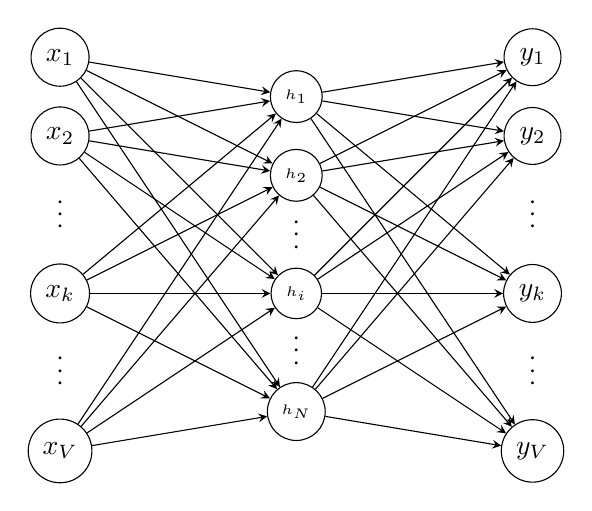
\begin{tikzpicture}[
          roundnode/.style={circle, draw=black, minimum size=4mm},
      ]

      \node[roundnode]   at (1,4)   (inputV)  {$x_V$};
      \node[roundnode]   at (1,6)   (inputK)  {$x_k$};
      \node[roundnode]   at (1,8)   (input2)  {$x_2$};
      \node[roundnode]   at (1,9)   (input1)  {$x_1$};

      \path (input2) -- (inputK) node [black, midway, sloped] {$\dots$};
      \path (inputK) -- (inputV) node [black, midway, sloped] {$\dots$};

      \node[roundnode]   at (4,4.5)   (hiddenN)  {\tiny $h_N$};
      \node[roundnode]   at (4,6)     (hiddenI)  {\tiny $h_i$};
      \node[roundnode]   at (4,7.5)   (hidden2)  {\tiny $h_2$};
      \node[roundnode]   at (4,8.5)   (hidden1)  {\tiny $h_1$};

      \path (hidden2) -- (hiddenI) node [black, midway, sloped] {$\dots$};
      \path (hiddenI) -- (hiddenN) node [black, midway, sloped] {$\dots$};

      \draw[-stealth] (input1) -- (hidden1);
      \draw[-stealth] (input1) -- (hidden2);
      \draw[-stealth] (input1) -- (hiddenI);
      \draw[-stealth] (input1) -- (hiddenN);
      \draw[-stealth] (input2) -- (hidden1);
      \draw[-stealth] (input2) -- (hidden2);
      \draw[-stealth] (input2) -- (hiddenI);
      \draw[-stealth] (input2) -- (hiddenN);
      \draw[-stealth] (inputK) -- (hidden1);
      \draw[-stealth] (inputK) -- (hidden2);
      \draw[-stealth] (inputK) -- (hiddenI);
      \draw[-stealth] (inputK) -- (hiddenN);
      \draw[-stealth] (inputV) -- (hidden1);
      \draw[-stealth] (inputV) -- (hidden2);
      \draw[-stealth] (inputV) -- (hiddenI);
      \draw[-stealth] (inputV) -- (hiddenN);


      \node[roundnode]   at (7,4)   (outputV)  {$y_V$};
      \node[roundnode]   at (7,6)   (outputI)  {$y_k$};
      \node[roundnode]   at (7,8)   (output2)  {$y_2$};
      \node[roundnode]   at (7,9)   (output1)  {$y_1$};

      \path (output2) -- (outputI) node [black, midway, sloped] {$\dots$};
      \path (outputI) -- (outputV) node [black, midway, sloped] {$\dots$};

      \draw[-stealth] (hidden1) -- (output1);
      \draw[-stealth] (hidden1) -- (output2);
      \draw[-stealth] (hidden1) -- (outputI);
      \draw[-stealth] (hidden1) -- (outputV);
      \draw[-stealth] (hidden2) -- (output1);
      \draw[-stealth] (hidden2) -- (output2);
      \draw[-stealth] (hidden2) -- (outputI);
      \draw[-stealth] (hidden2) -- (outputV);
      \draw[-stealth] (hiddenI) -- (output1);
      \draw[-stealth] (hiddenI) -- (output2);
      \draw[-stealth] (hiddenI) -- (outputI);
      \draw[-stealth] (hiddenI) -- (outputV);
      \draw[-stealth] (hiddenN) -- (output1);
      \draw[-stealth] (hiddenN) -- (output2);
      \draw[-stealth] (hiddenN) -- (outputI);
      \draw[-stealth] (hiddenN) -- (outputV);

  \end{tikzpicture}
  \caption{CBOW con 1 palabra por contexto}
  \label{redneuronal:3}
\end{figure}

En la figura \ref{redneuronal:3}, se muestra la versión simplificada de la red neuronal, donde el tamaño del vocabulario es $V\in\mathbb{N}$ y el tamaño de la capa escondida es $N\in\mathbb{N}$.
Las unidades entre capas adyacentes están conectadas totalmente a todas las unidades de la otra capa y viceversa. Como input de la red se usa un \textit{one-hot encoded vector},
que simplemente es un vector de tamaño $V$ donde cada posición representa una palabra. Es decir, si arbitrariamente, se deduce que la palabra 'coche` se va a representar en la $k-$ésima
posición, entonces el vector $(0, \dots, 1, \dots, 0)$ con un 1 en la $k-$ésima posición, sería la representación de la palabra coche.

Los pesos entra la capa de entrada y la de salida pueden ser representados por una matriz $W\in\mathbb{R}^{V\times N}$, donde cada fila de $W$ es la representación
vectorial $N-$dimensional de la palabra $w$ asociada en la capa de entrada. Las filas de esta matriz son la representación vectorial $N$-dimensional, $v_{w_I}$ (donde $I\in\{1, \ldots, V\}$),
de la palabra $w$ de entrada (representada por $x$).

Dado entonces un contexto con una única palabra, $w_I$, se tiene su representación como vector de entrada $x\in\mathbb{R}^V$, de forma que $x_k=1$ con $x_{k'}=0$ si $k'\neq k$. A partir de
$W$ y $x$, se puede obtener el vector $N$-dimensional de la capa intermedia, de la siguiente forma:
\begin{equation}\label{eq:h}
  h=W^Tx=W^T_{k, \cdot}=v^T_{w_I}
\end{equation}
donde es importante resaltar que esta operación no es más que copiar la fila $k$-ésima de $W$ en $h$. Esa fila fue denotada en el párrafo anterior por $v_{w_I}$.
Esto significa que la función de activación de la capa escondida es simplemente lineal, es decir, pasa directamente la suma ponderada de sus inputs a la siguiente capa.

De forma similar, se puede operar de la capa escondida a la capa de salida, donde se tiene una matriz de pesos diferente, $W'\in\mathbb{R}^{N\times V}$. En esta matriz, la representación
de cada palabra viene dada por cada una de sus columnas, es decir, la representación de la palabra $w_j$ en $W'$, es la columna $j$-ésima de $W'$ y es representada por $v'_{v_{w_j}}$. Con
esta notación, se puede calcular ahora un escalar (antes se ha calculado un vector) $u_j$ para cada una de las palabras del vocabulario:
\begin{equation}\label{eq:uj}
  u_j = v_{w_j}^{'T}h
\end{equation}
Finalmente, se puede usar \textit{softmax}, un modelo de clasificación lineal logarítmico, para obtener una distribución de las palabras (que es una distribución multinomial):
\begin{equation}\label{eq:yj}
p(w_j|w_I) = \frac{\exp(u_j)}{\sum_{j'=1}^V\exp(u_{j'})} =: y_j
\end{equation}
donde $y_j$ es el valor de la $j$-ésima neurona de la capa de salida. Una vez se tiene esta expresión, se pueden sustituir los valores de $u_j$ y $u_j'$ por los obtenidos
en párrafos anteriores, llegando a la siguiente fórmula:
\begin{equation}\label{eq:4}
  p(w_j|w_I) = \frac{\exp(w^{'T}_{w_j}v_{w_I})}{\sum_{j'=1}^V\exp(v^{'T}_{w_{j'}}v_{w_I})}
\end{equation}

Como clarificación, es importante recordar que $v_w$ y $v'_w$, son representaciones distintas de la palabra $w$:
\begin{itemize}
  \item $v_w$ proviene de las filas de la matriz $W$. Normalmente es denominado el vector de entrada.
  \item $v'_w$ proviene de las columnas de la matriz $W'$. Normalmente es denominado el vector de salida.
\end{itemize}

\subsubsection*{Actualización de pesos de capa escondida a capa de salida}

A continuación se presenta el desarrollo para la ecuación de actualización de pesos de este modelo. El objetivo de
entrenamiento (para una muestra de entrenamiento) es maximizar \ref*{eq:4}, que no es más que la probabilidad condicionada
de observar una palabra $w_O$ (denotando a su índice en la capa de salida por $j^*$), dada la palabra del contexto $w_I$:
\begin{equation}
  \begin{split}
  \max p(w_O|w_I) & = \max y_{j^*}\\
         & =\max \log(y_{j^*})\\
         & = u_{j^*} - \log \sum_{j'=1}^V\exp(u_{j'}) := -E \\
  \end{split}
\end{equation}
de donde se deduce que $E=-\log p(w_O|w_I)$ es la función de pérdida del modelo (porque es la función que se quiere minimizar).

Ahora es posible deducir la equación de actualización de pesos entre la capa escondida y la de salida. Para ello, se calcula
la derivada de $E$ respecto al escalar $u_j$, que se definió anteriormente para cada palabra:
\begin{equation}
  \begin{split}
  \frac{\partial E}{\partial u_j} & = \left(-u_{j*}+ \log\sum_{j'=1}^V\exp(u_{j'})\right)\frac{\partial}{\partial u_j} \\
  \end{split}
\end{equation}
Para el desarrollo de esa expresión, es importante resaltar que $j^*\neq j$, por lo que la expresión resultante queda mucho
más simple:
\begin{equation}
  \frac{\partial E}{\partial u_j} = y_j - t_j, \;\; \forall j \in \{1, \cdots, V\}
\end{equation}
donde $y_j$ fue definido en \ref*{eq:yj} y $t_j$ es definido, por simplicidad, como:
\[ t_j = \begin{cases}
  1 & j = j^* \\
  0 & j \neq j^*
\end{cases}
\]
Es importante notar que lo que se acaba de calcular no es más ni menos que la componente $j$-ésima del error de predicción de la capa de salida, por lo tanto,
se puede notar como:
\begin{equation}\label{eq:ej}
  \frac{\partial E}{\partial u_j} = y_j - t_j := e_j, \;\; \forall j \in \{1, \cdots, V\}
\end{equation}
Ahora es necesario calcular el gradiente en los pesos entre la capa escondida y de salida (que fueron denotados por $W'=\{w'_{ij}\}$). Para ello,
basta con derivar la misma expresión pero respecto de $w'_{ij}$:
\begin{equation}
  \frac{\partial E}{\partial w'_{ij}} = \frac{\partial E}{\partial u_j} \frac{\partial u_j}{\partial w'_{ij}} = e_j h_i
\end{equation}
Por lo tanto, ya se puede aplicar la técnica de descenso de gradiente porque se ha obtenido la ecuación de actualización de pesos para cada uno de los valores de $W'$:
\[
  w_{ij}^{(nuevo)} = w_{ij}^{'(viejo)} - \eta e_jh_i
\]
En lugar de escalar a escalar, esa expresión también se puede escribir usando la representación vectorial de la palabra $w$ en $W'$, es decir, $v'_{w_j}$:
\[
  v_{w_j}^{'(nuevo)}= v_{w_j}^{'(viejo)} - \eta e_j h, \;\;\; j \in \{1, \cdots, V\}
\]
donde $\eta > 0$ es el ratio de aprendizaje.

Es importante resaltar que esta ecuación implica que es necesario recorrer cada posible palabra en el vocabulario, comprobar su probabilidad de la capa de salida, $y_j$, y
compararlo con su valor esperado, $t_j$ (que solo puede ser 0 o 1). Si se da $y_j > t_j $ (caso de sobreestimación) entonces se resta una proporción de $h$ (se recuerda que
$h=v_{w_I}$) a $v'_{w_j}$. Si se tiene el caso contrario, entonces se realiza la operación contraria. En ambos casos, $v'_{w_O}$ es cada vez más cercano a $v_{w_I}$ (en
este caso la \textit{cercanía} usa el producto escalar y no la distancia euclídea usual).

\subsubsection*{Actualización de pesos de capa de entrada a capa escondida}

Una vez obtenida la ecuación para actualizar los pesos de la capa escondida a la de salida, se pueden usar usar esos mismos cálculos para calcular
la ecuación de actualización de la capa anterior (\textit{back-propagation}), es decir, de la capa de entrada a la de salida.

Para obtener esa ecuación, es necesario minimizar una vez más la función de error $E$, pero esta vez con respecto a $h_i$:
\begin{equation}
  \frac{\partial E}{\partial h_i} = \sum_{j=1}^V\frac{\partial E}{\partial u_j} \frac{\partial u_j}{\partial h_i} = \sum_{j=1}^Ve_j w'_{ij} := EH_i, \;\; \forall i \in \{1, \cdots, N\}
\end{equation}
donde $h_i$ es la $i$-ésima componente de la capa escondida, $u_j$ se definió en \ref*{eq:uj} y $e_j$ se definió en \ref*{eq:ej} como el error de predicción
de la $j$-ésima unidad de la capa de salida. A partir de $EH_i$, se puede definir un vector de dimensión $N$, en el que cada componente es la suma de los vectores
de salida de todas las palabras, promediados por el error de predicción.

El siguiente paso sería calcular la derivada de $E$ con respecto de $W$. Primero, se recuerda que la capa escondida simplemente es una función lineal de los valores de la capa de entrada. Expandiendo
la notación vectorial de \ref*{eq:h}, se obtiene:
\begin{equation}
  h_i=\sum_{k=1}^Vx_kw_{ki}
\end{equation}
Usando esa expresión se puede derivar $E$ con respecto a cada elemento de $W$, obteniendo:
\begin{equation}
  \frac{\partial E}{\partial w_{ki}} = \frac{\partial E}{\partial h_i} \frac{\partial h_i}{\partial w_{ki}} = EH_i x_k
\end{equation}
Con ese resultado, se puede expresar $\frac{\partial E}{\partial W}=xEH^T$. Como solo un componente de $x$ es distinto de cero (se recuerda que se están usando \textit{one-hot encoded vectors}), solo
una fila de $\frac{\partial E}{\partial W}$ es distinta de cero, y su valor es $EH^T$, un vector $N$-dimensional.  Finalmente, se puede obtener la ecuación de actualización de $W$:
\begin{equation}
  v_{w_I}^{(nuevo)} = v_{w_I}^{(antiguo)} - \eta EH^T
\end{equation}
donde $v_{w_I}$ es una fila de $W$, la representación del vector de entrada (la única palabra del contexto). Como consecuencia de que solo una fila de $\frac{\partial E}{\partial W}$ sea distinta de 0,
es que todas las otras filas de $W$ permanecerán sin cambiar después de esta iteración.

De igual forma que en el apartado anterior, si la probabilidad de una palabra $w_j$ es sobreestimada ($y_j>t_j$), entonces el vector de entrada de la palabra del contexto $w_I$ tenderá a alejarse del vector de salida
de $w_j$. Lo contrario es cierto, si la probabilidad es subestimada. Por lo tanto, el movimiento del vector de entrada de $w_I$ es determinado por el error de predicción de todos los vectores en el vocabulario. Cuanto más
grande sea el error de predicción, más significativo será el cambio en el vector de entrada de la palabra del contexto.

Conforme se actualizan los parámetros del modelo de forma iterativa, los efectos de cada iteración se van a ir acumulando. Se puede imaginar que el vector de salida de una palabra $w$ es `arrastrado' de un lado hacia otro
por los vectores de entrada de los vecinos de $w$.
\subsection{Contexto de múltiples palabras}

La figura \ref{redneuronal:4} muestra el modelo en el caso de varias palabras por contexto. Cuando se calcula la salida de la capa
escondida, en lugar de copiar directamente el valor del vector de entrada de la palabra del contexto, el modelo calcula la media
de todos los vectores de las palabras en el contexto, resultando en la siguiente expresión de $h$:
\begin{equation}
  \begin{split}
     h & = \frac{1}{C} W^T \left( x_1 + x_2 + \cdots + x_C \right)\\
       & = \frac{1}{C} \left( v_{w_1} + v_{w_2} + \cdots + v_{w_C} \right)^T\\
    \end{split}
\end{equation}
donde $C$ es el número de palabras en el contexto, $w_1, \cdots, w_C$ son las palabras en el contexto y $v_w$ es la representación de entrada
de una palabra $w$. En este caso particular, repitiendo los cálculos del apartado anterior, se obtiene la siguiente función de pérdida:
\begin{equation}
  \begin{split}
    E & = -\log p\left( w_O | w_{I,1}, \cdots, w_{I, C} \right) \\
      & = -u_j^* + \log\displaystyle\sum_{j'=1}^V\exp\left(u'_j\right) \\
      & = -v_{w_O}^{'T}h + \log\displaystyle\sum_{j'=1}^V\exp\left( v_{w_j}^{'T}h \right) \\
  \end{split}
\end{equation}

\begin{figure}[ht]
  \centering
  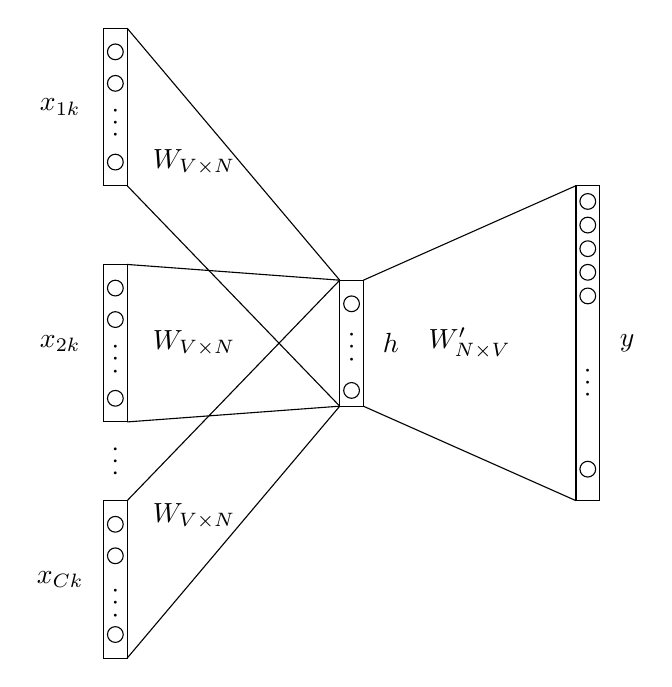
\begin{tikzpicture}[
          roundnode/.style={circle, draw=black, minimum size=4mm},
      ]

      \node[rectangle, draw, minimum width = 0.3cm, minimum height = 2cm] (xck) at (0.5,0) {};
      \node[] at (-0.2,0) {$x_{Ck}$};
      \draw[] (0.5, 0.7) circle (0.1cm);
      \draw[] (0.5, 0.3) circle (0.1cm);
      \draw[] (0.5, -0.7) circle (0.1cm);
      \path (0.5, -0.9) -- (0.5, 0.3) node [black, midway, sloped] {$\dots$};

      \node[rectangle, draw, minimum width = 0.3cm, minimum height = 2cm] (xdk) at (0.5,3) {};
      \node[] at (-0.2,3) {$x_{2k}$};
      \draw[] (0.5, 3.7) circle (0.1cm);
      \draw[] (0.5, 3.3) circle (0.1cm);
      \draw[] (0.5, 2.3) circle (0.1cm);
      \path (0.5, 2.3) -- (0.5, 3.3) node [black, midway, sloped] {$\dots$};

      \node[rectangle, draw, minimum width = 0.3cm, minimum height = 2cm] (xuk) at (0.5,6) {};
      \node[] at (-0.2,6) {$x_{1k}$};
      \draw[] (0.5, 6.7) circle (0.1cm);
      \draw[] (0.5, 6.3) circle (0.1cm);
      \draw[] (0.5, 5.3) circle (0.1cm);
      \path (0.5, 5.3) -- (0.5, 6.3) node [black, midway, sloped] {$\dots$};

      \path (xdk) -- (xck) node [black, midway, sloped] {$\dots$};

     % ========= hidden layer


      \node[rectangle, draw, minimum width = 0.3cm, minimum height = 1.6cm] (xdk) at (3.5,3) {};
      \node[] at (4,3) {$h$};
      \draw[] (3.5, 3.5) circle (0.1cm);
      \draw[] (3.5, 2.4) circle (0.1cm);
      \path (3.5, 2.4) -- (3.5, 3.5) node [black, midway, sloped] {$\dots$};

     % ========= connections input->hidden layer

     \draw[] (0.65,1) -- (3.35,3.8);
     \draw[] (0.65,4) -- (3.35,3.8);
     \draw[] (0.65,7) -- (3.35,3.8);

     \draw[] (0.65,-1) -- (3.35,2.2);
     \draw[] (0.65,2) -- (3.35,2.2);
     \draw[] (0.65,5) -- (3.35,2.2);

     \node[] at (1.5,0.8) {$W_{V\times N}$};
     \node[] at (1.5,3) {$W_{V\times N}$};
     \node[] at (1.5,5.3) {$W_{V\times N}$};


     % ========= output layer

     \node[rectangle, draw, minimum width = 0.3cm, minimum height = 4cm] (xdk) at (6.5,3) {};
     \node[] at (7,3) {$y$};
     \draw[] (6.5, 4.8) circle (0.1cm);
     \draw[] (6.5, 4.5) circle (0.1cm);
     \draw[] (6.5, 4.2) circle (0.1cm);
     \draw[] (6.5, 3.9) circle (0.1cm);
     \draw[] (6.5, 3.6) circle (0.1cm);
     \draw[] (6.5, 1.4) circle (0.1cm);
     \path (6.5, 1.4) -- (6.5, 3.6) node [black, midway, sloped] {$\dots$};


     % ========= connections hidden->output layer

     \draw[] (3.65,3.8) -- (6.35, 5);
     \draw[] (3.65,2.2) -- (6.35, 1);

     \node[] at (5,3) {$W'_{N\times V}$};

  \end{tikzpicture}
  \caption{CBOW con C palabras por contexto}
  \label{redneuronal:4}
\end{figure}

La ecuación de actualización de la capa escondida a la de salida, es básicamente la misma que para el contexto de una
única palabra (pero ahora $h$ ha sido definida de diferente forma):
\begin{equation}
  v_{w_j}^{'(nuevo)}=v_{w_j}^{'(viejo)} - \eta e_j h, \;\;\; j \in \{1, \cdots, V\}
\end{equation}
Es importante notar que es necesario aplicar esta ecuación a cada elemento de la matriz de pesos de la capa escondida a la de salida,
por cada iteración en el entrenamiento del modelo.

La ecuación de actualización para la capa de entrada a la escondida es similar a la de una palabra por contexto, excepto que ahora es
necesario aplicarlo para cada palabra $w_{I,c}$ en el contexto:
\begin{equation}
  v_{w_{I,c}}^{(nuevo)} = v_{w_{I,c}}^{(antiguo)} - \frac{1}{C}\eta EH^T \;\; \forall c \in \{1,2,\cdots, C \}
\end{equation}

\subsection{Extensión a tropos}

Una vez el modelo se ha desarrollado completamente, se puede realizar la extensión a datos que no sean palabras, como por ejemplo, tropos. La principal distinción
entre las palabras y los tropos es el orden. En una oración el orden de las palabras tiene gran importancia porque determina en cierto sentido parte de su significado. Por
el contrario, en una película u obra cultural, los tropos no tienen un orden definido. Por ejemplo, pueden darse dos o más tropos al mismo tiempo.

En el desarrollo matemático anterior se puede observar que lo único que se ha usado para representar el orden de las palabras es el contexto. Por lo tanto, para no considerar el orden,
lo único que hay que hacer es incrementar el tamaño del contexto al del vocabulario, quedando:

\begin{equation}
  h = W^T(x_1+x_2+\cdots + x_V) = \sum_{i=1}^V v_{w_i}
\end{equation}

\begin{equation}
  v_{w_{I,i}}^{(nuevo)} = v_{w_{I,i}}^{(antiguo)} - \frac{1}{V}\eta EH^T \;\; \forall i \in \{1,2,\cdots, V \}
\end{equation}

\begin{equation}
  v_{w_j}^{'(nuevo)}=v_{w_j}^{'(viejo)} - \eta e_j h, \;\;\; j \in \{1, \cdots, V\}
\end{equation}

Las expresiones de $E$ y $EH$ no han cambiado, ya que no dependían del contexto.

\section{Skip-gram}

Esta versión del modelo fue introducida en \cite{word2vec:1} \cite{word2vec:2}. En la figura \ref{redneuronal:5} se muestra el modelo. Como se
puede apreciar, es la versión contrario al modelo de bolsa continua de palabras. En este caso solo tenemos una palabra de entrada y $C$ de salida (las
del contexto).

Se va a seguir denotando por $v_{w_I}$ al único vector de entrada en la capa de entrada. Además se tiene la misma definición de $h$ \ref{eq:h}. Se recuerda que $h$
no era más que copiar y transponer una fila de $W$:
\[
  h = W_{(k,\cdot)}^T := w_{w_i}^T
\]

\begin{figure}[ht]
  \centering
  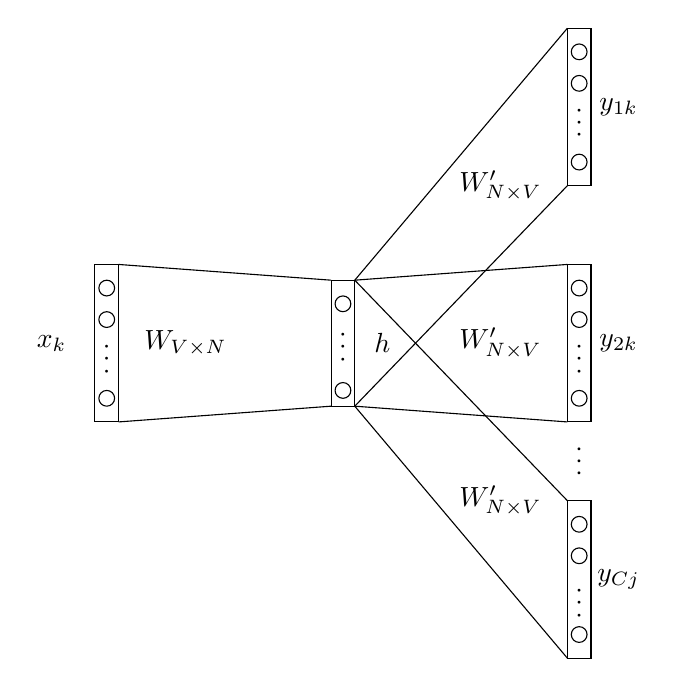
\begin{tikzpicture}[
          roundnode/.style={circle, draw=black, minimum size=4mm},
      ]
      \node[rectangle, draw, minimum width = 0.3cm, minimum height = 2cm] (xk) at (0.5,3) {};
      \node[] at (-0.2,3) {$x_{k}$};
      \draw[] (0.5, 3.7) circle (0.1cm);
      \draw[] (0.5, 3.3) circle (0.1cm);
      \draw[] (0.5, 2.3) circle (0.1cm);
      \path (0.5, 2.3) -- (0.5, 3.3) node [black, midway, sloped] {$\dots$};

      \node[rectangle, draw, minimum width = 0.3cm, minimum height = 1.6cm] (xdk) at (3.5,3) {};
      \node[] at (4,3) {$h$};
      \draw[] (3.5, 3.5) circle (0.1cm);
      \draw[] (3.5, 2.4) circle (0.1cm);
      \path (3.5, 2.4) -- (3.5, 3.5) node [black, midway, sloped] {$\dots$};

    %  % ========= connections input->hidden layer

     \draw[] (0.65,4) -- (3.35,3.8);
     \draw[] (0.65,2) -- (3.35,2.2);

     \node[] at (1.5,3) {$W_{V\times N}$};


    %  % ========= output layer

      \node[rectangle, draw, minimum width = 0.3cm, minimum height = 2cm] (ycj) at (6.5,0) {};
      \node[] at (7,0) {$y_{Cj}$};
      \draw[] (6.5, 0.7) circle (0.1cm);
      \draw[] (6.5, 0.3) circle (0.1cm);
      \draw[] (6.5, -0.7) circle (0.1cm);
      \path (6.5, -0.9) -- (6.5, 0.3) node [black, midway, sloped] {$\dots$};

    \node[rectangle, draw, minimum width = 0.3cm, minimum height = 2cm] (ydj) at (6.5,3) {};
    \node[] at (7,3) {$y_{2k}$};
    \draw[] (6.5, 3.7) circle (0.1cm);
    \draw[] (6.5, 3.3) circle (0.1cm);
    \draw[] (6.5, 2.3) circle (0.1cm);
    \path (6.5, 2.3) -- (6.5, 3.3) node [black, midway, sloped] {$\dots$};

    \node[rectangle, draw, minimum width = 0.3cm, minimum height = 2cm] (yuj) at (6.5,6) {};
    \node[] at (7,6) {$y_{1k}$};
    \draw[] (6.5, 6.7) circle (0.1cm);
    \draw[] (6.5, 6.3) circle (0.1cm);
    \draw[] (6.5, 5.3) circle (0.1cm);
    \path (6.5, 5.3) -- (6.5, 6.3) node [black, midway, sloped] {$\dots$};

    \path (ydj) -- (ycj) node [black, midway, sloped] {$\dots$};

    %  % ========= connections hidden->output layer

     \draw[] (3.65,3.8) -- (6.35, 7);
     \draw[] (3.65,2.2) -- (6.35, 5);

     \draw[] (3.65,3.8) -- (6.35, 4);
     \draw[] (3.65,2.2) -- (6.35, 2);

     \draw[] (3.65,3.8) -- (6.35, 1);
     \draw[] (3.65,2.2) -- (6.35, -1);

     \node[] at (5.5,5) {$W'_{N\times V}$};
     \node[] at (5.5,3) {$W'_{N\times V}$};
     \node[] at (5.5,1) {$W'_{N\times V}$};

  \end{tikzpicture}
  \caption{Skip-gram con C palabras por contexto}
  \label{redneuronal:5}
\end{figure}

Ahora, en la capa de salida, en lugar de tener una distribución multinomial lo que se tiene son $C$ distribuciones
multinomiales. Cada salida se calcula usando la misma matriz $W'$:
\[
  p\left( w_{c,j} = w_{O,c} | w_I \right) = y_{c,j} = \frac{\exp(u_{c,j})}{\sum_{j'=1}^V\exp(u_{j'})}
\]
donde $w_{c,j}$ es la $j$-ésima palabra del $c$-ésimo elemento en la capa de salida; $w_{O,c}$ es la $c$-ésima
palabra en el contexto; $w_I$ es la única palabra de entrada; $y_{c,j}$ es la salida de la $j$-ésima unidad en la $c$-ésima
palabra de la capa de salida; $u_{c,j}$ es el valor de la red de la $j$-ésima unidad en la $c$-ésima palabra de la capa de salida.
Como cada palabra de la capa de salida usa la misma matriz de pesos $W'$, se tiene:
\[
  u_{c,j} = u_j = v^{'T}_{w_j}h \;\;\; c=1,\cdots, C
\]
donde $v'_{w_j}$ es el vector de salida de la $j$-ésima palabra en el vocabulario, $w_j$. Además, $v'_{w_j}$ no es más que una de las
columnas de la matriz de pesos $W'$.

La derivación de las ecuaciones de actualización no es muy diferente del proceso desarrollado en el modelo anterior. Simplemente se cambia la función de pérdida a:
\begin{align}
  E & = - \log p\left( w_{O,1}, w_{O,2}, \cdots, w_{O,C} | w_I \right) \\
    & = - \log \prod_{c=1}^C \frac{\exp(u_{c,j_c^*})}{\sum_{j'=1}^V\exp(u_{j'})} \\
    & = - \sum_{c=1}^C u_{j^*_c} + C\log \sum_{j'=1}^V\exp(u_{j'}).
\end{align}
donde $j_c^*$ es el índice de la $c$-ésima palabra del contexto en el vocabulario.

Ahora se deriva $E$ respecto al valor de la red $u_{c,j}$:
\[
  \frac{\partial E}{\partial u_{c,j}} = y_{c,j} - t_{c,j} := e_{c,j}
\]
que es el error de predicción de cada unidad. Para simplificar la notación se define un vector $V$-dimensional $EI=\{EI_1, \cdots, EI_V\}$ como la suma de los errores de
predicción sobra todas las palabras del contexto:
\[
  EI_j = \sum_{c=1}^C e_{c,j}
\]
A continuación, se calcula la derivada de $E$ con respecto a cada elemento de $W'$, obteniendo:
\[
  \frac{\partial E}{\partial w'_{ij}} = \sum_{c=1}^C \frac{\partial E}{\partial u_{c,j}} \frac{\partial u_{c,j}}{\partial w'_{ij}} = EI_j h_i
\]
Con lo que se han obtenido las ecuaciones de actualización para la capa escondida y la capa de salida:
\[
w_{ij}^{'(nueva)} = w_{ij}^{'(vieja)} - \eta EI_j h_i
\]
o
\[
  v_{w_{j}}^{'(nueva)}= v_{w_j}^{'(vieja)} - \eta EI_j h \;\;\; j = 1,2, \cdots, V
\]
La obtención de la ecuación de actualización para la capa de entrada y escondida es igual que en el modelo anterior, obteniéndose:
\[
  v_{w_I}^{(nueva)} = w_{w_I}^{(vieja)} - \eta EH^T
\]
donde $EH$ es un vector $N$-dimensional, donde cada componente viene definida por:
\[
  EH_i = \sum_{j=1}^V EI_j w_{ij}'
\]

\subsection{Extensión a tropos}

De igual forma se puede proceder en esta versión del modelo y eliminar el orden para poder usar datos como tropos. En este caso, la función de pérdida
sí que ha sufrido cambios:
\begin{align}
  E & = - \log p\left( w_{O,1}, w_{O,2}, \cdots, w_{O,V} | w_I \right) \\
    & = - \log \prod_{i=1}^V \frac{\exp(u_i)}{\sum_{j'=1}^V\exp(u_{j'})} \\
    & = - \sum_{j=1}^V u_{j} + V\log \sum_{j'=1}^V\exp(u_{j'}).
\end{align}

En este caso la expresión de $h$ no cambia ya que siempre se ha tenido una palabra únicamente, independientemente del contexto. Por lo
tanto, el valor de la unidad $u_{j}$ tampoco ha cambiado. Las expresiones de $v$ y $v'$ tampoco han sufrido alteraciones adicionales.

\section{\textit{Softmax} jerárquico}

Como se puede deducir a partir de \ref{eq:yj}, calcular el denominador de la función \textit{softmax} es increíblemente caro. Para disminuir el tiempo de ejecución de ese cálculo
se pueden aplicar dos técnicas:

\begin{itemize}
  \item Muestreo negativo \cite{goldberg2014word2vec}: en esta técnica se genera el par esperado (o positivo). Posteriormente se escojen $k$ muestras adicionales, que no se generan a partir del contexto, es decir, son \textit{negativas}.
  Una vez se tienen las muestras positivas y negativas, se aplica una nueva función objetivo más rápida de calcular que \textit{softmax}. Esta opción se ha descartado porque en el caso de tropos no
  está muy claro cómo se deberían generar esas muestras negativas.
  \item \textit{Softmax} jerárquico: esta opción evita usar todo el vocabulario en cada cálculo, usando solo un número muy reducido de elementos del vocabulario. Esta opción se desarrolla a continuación.
\end{itemize}

El algoritmo \textit{softmax jerárquico} es una forma eficiente de calcular la función \textit{softmax} \cite{morin2005hierarchical}. El algoritmo usa un árbol binario para representar todos los términos
del vocabulario (de su representación en vectores). Si el vocabulario tiene $V$ términos, el árbol tendrá $V$ nodos hoja, uno por cada término. Es fácil comprobar que en un árbol binario se tienen $V-1$ nodos intermedios (el árbol binario
usado es de Huffman, así cada nodo interno tiene siempre dos hijos \cite{van1976construction}).
Por cada nodo hoja, existe un camino único desde la raíz hasta dicha hoja. Ese camino es usado para estimar la probabilidad de la palabra representada por la hoja. En la figura REFERENCIAR se puede apreciar un
ejemplo:

%% INCLUIR AQUI FIGURA

Un hecho importante de usar este algoritmo es que se pierde la representación de los vectores de salida. En su lugar, cada uno de los $V-1$ nodos intermedios tiene un vector de salida asociado
$v'_{n(w,j)}$. La función objetivo cambia considerablemente, siendo ahora la probabilidad de que un término sea el término de salida:
\begin{equation}\label{eq:soft}
  p\left( w=w_O \right) = \prod_{j=1}^{L(w)-1}\sigma\left( \llbracket n(w, j+1)=ch(n(w,j))\rrbracket v^{'T}_{n(w,j)}h \right)
\end{equation}

donde $ch(n)$ es el hijo izquierdo del nodo $n$; $v'_{n(w,j)}$ es la representación del nodo $n(w,j)$; $h$ es el valor de salida de la capa escondida; $\llbracket x\rrbracket$ es una función especial
definida como:
\begin{equation}
  \llbracket x \rrbracket = \begin{cases}
    1 & \text{ si x es cierto} \\
    -1 & \text{ si x es falso}
  \end{cases}
\end{equation}

Véase un ejemplo para comprender un poco más esta nueva función. Mirando la figura REFERENCIAR, supóngase que se quiere calcular la probabilidad de $w_2$ siendo el término de salida. Se define esa
probabilidad como la probabilidad de un camino aleatorio empezando desde la raíz y terminando en el nodo hoja de $w_2$. En cada nodo interno (incluyendo la raíz), es necesario asignar las probabilidades
de ir hacia la izquierda o hacia la derecha. La probabilidad de ir hacia la izquierda se define como:
\begin{equation}
  p\left( n, izquierda \right) = \sigma\left( v^{'T}_n h \right)
\end{equation}

que es determinada por la representación vectorial del nodo interno y el valor de la capa de salida (que es a su vez determinado por la representación vectorial del término de entrada). De forma sencilla
se puede calcular la probabilidad de ir hacia la derecha:
\begin{equation}
  p\left( n, derecha \right) = 1 - p\left( n, izquierda \right) = \sigma\left( v^{'T}_n h \right)
\end{equation}

Siguiendo el camino en la figura REFERENCIAR, del nodo raíz a $w_2$, se puede calcular la probabilidad buscada:
\begin{align}
  p\left( w_2 = w_O \right) & = p\left( n(w_2, 1), izquierda \right) p\left( n(w_2, 2), izquierda \right) p\left(n(w_2, 3), derecha\right)\\
                            & = \sigma\left( v^{'T}_{n(w_2, 1)h} \right) \sigma\left( v^{'T}_{n(w_2, 2)h} \right) \sigma\left( - v^{'T}_{n(w_2, 3)h} \right)
\end{align}

que es exactamente lo que se obtiene desarrollando \ref{eq:soft}. De igual forma, teniendo en cuenta la definición de $\sigma$, es fácil ver que:
\begin{equation}
  \sum_{i=1}^Vp\left( w_i = w_O \right) = 1
\end{equation}

haciéndo que al \textit{softmax jerárquico} una distribución multinomial bien definida.

Ahora lo que queda es escribir las nuevas ecuaciones de actualización. Por simplicidad primero se va a proceder con el modelo de un término por contexto, ya que extenderlas
al de más términos, es muy sencillo. Para simplificar la notación, se toma:
\begin{equation}
  \llbracket \dot \rrbracket := \llbracket  n(w, j+1) = ch(n(w,j)) \rrbracket
\end{equation}
\begin{equation}
  v'_j := v'_{n_{w,j}}
\end{equation}
La función de error con la nueva probabilidad viene definida por:
\begin{equation}
  E = - \log p\left( w=w_O|w_I \right) = - \sum_{j=1}^{L(w) - 1} \log\sigma\left( \llbracket \dot \rrbracket v^{'T}_jh \right)
\end{equation}
Derivando $E$ respecto de $v'_jh$, se obtiene:
\begin{align}
  \frac{\partial E}\partial v'_j h{} & = \left( \sigma\left( \llbracket \dot \rrbracket v^{'T}_jh \right) \right) \llbracket \dot \rrbracket \\
                                     & = \begin{cases}
                                      \sigma\left( \llbracket \dot \rrbracket v^{'T}_jh \right) - 1 & (\llbracket \dot \rrbracket = 1) \\
                                      \sigma\left( \llbracket \dot \rrbracket v^{'T}_jh \right) & (\llbracket \dot \rrbracket = -1)
                                    \end{cases} \\
                                    & = \sigma\left( \llbracket \dot \rrbracket v^{'T}_jh \right) - t_j
\end{align}
donde $t_j=1$ si $\llbracket \dot \rrbracket = 1$ y $t_j=0$ en otro caso. A continuación se deriva $E$ con respecto a la representación vectorial del nodo interno $n(w,j)$, obteniendo:
\begin{equation}
  \frac{\partial E}{\partial v'_j} = \frac{\partial E}{\partial v'_j h} \frac{\partial v'_jh}{\partial v'_j} = \left( \sigma\left( v^{'T}_j h \right) - t_j \right) h
\end{equation}
Lo que produce la siguiente ecuación de actualización:
\begin{equation}
  v^{'(nuevo)}_j = v^{'(viejo)}_j - \nabla \left( \sigma\left( v^{'T}_j h \right) - t_j \right)h
\end{equation}
Para propagar el error, simplemente hay que tomar la derivdada de $E$ con respecto a $h$:
\begin{align}
  \frac{\partial E }{\partial h} & = \sum_{j=1}^{L(w) - 1}\frac{\partial E}{\partial v'_jh} \frac{\partial v'_jh}{\partial h} \\
                                 & = \sum_{j=1}^{L(w) - 1} \left( \sigma\left( v^{'T}_j h \right) - t_j \right)v'_j \\
                                 & := EH
\end{align}
Basta con sustituir la nueva expresión de $EH$ en las ecuaciones que ya se tenían.

A partir de las ecuaciones de actualización se puede observar que la complejidad computacional ha pasado de $O(V)$ a $O(\log V)$, lo que implica una gran mejora
en velocidad. Sin embargo, todavía se tienen más o menos la misma cantidad de parámetros: $V-1$ frente a los $V$ anteriores.